\documentclass[12pt, titlepage]{article}

\usepackage{fullpage}
\usepackage[round]{natbib}
\usepackage{multirow}
\usepackage{booktabs}
\usepackage{tabularx}
\usepackage{graphicx}
\usepackage{float}
\usepackage{xcolor}
\usepackage{soul}
\usepackage{hyperref}
\hypersetup{
    colorlinks,
    citecolor=black,
    filecolor=black,
    linkcolor=red,
    urlcolor=blue
}
\usepackage[round]{natbib}

\newcounter{acnum}
\newcommand{\actheacnum}{AC\theacnum}
\newcommand{\acref}[1]{AC\ref{#1}}

\newcounter{ucnum}
\newcommand{\uctheucnum}{UC\theucnum}
\newcommand{\uref}[1]{UC\ref{#1}}

\newcounter{mnum}
\newcommand{\mthemnum}{M\themnum}
\newcommand{\mref}[1]{M\ref{#1}}

\title{SE 3XA3: Module Guide\\Google Images Downloader}

\author{Team \#201, CAS Dream Team
		\\ Sam Crawford, crawfs1, 400129435
		\\ Joshua Guinness, guinnesj, 400134735
		\\ Nicholas Mari, marin, 400132494
}

\date{\today}

% \input{../../Comments}

\begin{document}

\maketitle

\pagenumbering{roman}
\tableofcontents
\listoftables
\listoffigures

\begin{table}[tp]
\begin{tabularx}{\textwidth}{llll}
\toprule {\bf Date} & {\bf Name} & {\bf Version} & {\bf Notes}\\
\midrule
2/26/2020 & Nick & 1.0 & Created document\\
3/9/2020 & Sam & 1.1 & Filled in admin details\\
3/9/2020 & Sam & 1.1.1 & Started adding modules\\
3/10/2020 & Josh, Sam, Nick & 1.1.2 & First iteration of all sections completed\\
3/11/2020 & Sam, Nick & 1.2 & Finishing touches\\
3/13/2020 & Josh & 1.2.1 & Finishing section 2, general edits\\
3/13/2020 & Nick & 1.2.2 & General edits\\
\textcolor{red}{4/6/2020} & \color{red}Sam & \color{red}2.0 & \color{red}Final revision for Rev 1\\
\bottomrule
\end{tabularx}
\caption{\bf Revision History}
\end{table}

%\begin{table}[bp]
%\caption{\bf Revision History}
%\begin{tabularx}{\textwidth}{p{3cm}p{2cm}X}
%\toprule {\bf Date} & {\bf Version} & {\bf Notes}\\
%\midrule
%3/9/2020 & 1.0 & Added\\
%Date 2 & 1.1 & Notes\\
%\bottomrule
%\end{tabularx}
%\end{table}

\newpage

\pagenumbering{arabic}

\section{Introduction}

The software system being developed is a google images downloader command line tool that
will allow end users to download a certain number of googles images given
specific keywords and parameters. The aim of this tool is to provide assistance to those
involved in machine learning, and secondarily those involved in art.

After completing the first stage of the design, the Software Requirements Specification (SRS), this document, the Module Guide (MG) is developed~\citep{ParnasEtAl1984}. The MG
specifies the modular structure of the system and is intended to allow both
designers and maintainers to easily identify the parts of the software. After the MG is completed, the Module Interface Specification will be done which specifies the externally observable behaviour of a module using precise mathematical language.

A module is a work assignment for a programmer or programming team~\citep{ParnasEtAl1984}. The primary design principle being followed when decomposing the system into modules is the principle of information hiding~\citep{Parnas1972a}. This principle supports design for change, because the ``secrets'' that each module hides represent likely future changes.

Other design principles follow the rules laid out by \citet{ParnasEtAl1984}. They are as follows:
\begin{itemize}
\item System details that are likely to change independently should be the
  secrets of separate modules.
\item Each data structure is used in only one module.
\item Any other program that requires information stored in a module's data
  structures must obtain it by calling access programs belonging to that module.
\end{itemize}

The rest of the document is organized as follows. Section
\ref{SecChange} lists the anticipated and unlikely changes of the software
requirements. Section \ref{SecMH} summarizes the module decomposition that
was constructed according to the likely changes. Section \ref{SecConnection}
specifies the connections between the software requirements and the
modules. Section \ref{SecMD} gives a detailed description of the
modules. Section \ref{SecTM} includes two traceability matrices. One checks
the completeness of the design against the requirements provided in the SRS. The
other shows the relation between anticipated changes and the modules. Section
\ref{SecUse} describes the use relation between modules.

\section{Anticipated and Unlikely Changes} \label{SecChange}

This section lists possible changes to the system that are classified into two
categories according to the likeliness of the change. Anticipated changes are 
listed in Section \ref{SecAchange}, and unlikely changes are listed in Section \ref{SecUchange}.
Table \ref{table:tracechanges} shows the traceability matrix between the anticipated changes and modules.

\subsection{Anticipated Changes} \label{SecAchange}

Anticipated changes are the source of the information that are to be hidden
inside the modules. This was, changing one of the anticipated changes will only
require changing the one module that hides the associated decision. The is called design for change.

\begin{description}
\item[\refstepcounter{acnum} \actheacnum \label{acHTMLStructure}:] Google Images will likely change the way that their HTML is structured in the future.
This will require a change in the Navigate Page Module.
\item[\refstepcounter{acnum} \actheacnum \label{acQueryFormat}:] Google Images will likely change the search query format, requiring a change 
in the Search Query Module.
\item[\refstepcounter{acnum} \actheacnum \label{acInputParam}:] Google Images may change the search paramaters available to use, resulting 
in a change in the Input Module.
\end{description}

\subsection{Unlikely Changes} \label{SecUchange}

These are changes that are unlikely to happen as changing them will likely require many parts of the design to 
be modified. This is obviously not ideal.

\begin{description}
\item[\refstepcounter{ucnum} \uctheucnum \label{ucIO}:] Input/Output devices
  (Input: File and/or Keyboard, Output: Images downloaded to a directory).
\item[\refstepcounter{ucnum} \uctheucnum \label{ucInput}:] The system will take in user input from either from the command line or from a file.
\item[\refstepcounter{ucnum} \uctheucnum \label{ucOutput}:] The system will download images to either a local folder, or a specified
location on a server.
\item[\refstepcounter{ucnum} \uctheucnum \label{ucOutput}:] The program will run on a computer or server that has the necessary tools 
downloaded and installed, not an embedded system.
\item[\refstepcounter{ucnum} \uctheucnum \label{ucFlow}:] The data flow and \st{logic of the system} \textcolor{red}{system architecture} is unlikely to change.
\end{description}

\newpage

\section{Module Hierarchy} \label{SecMH}

This section provides an overview of the module design. Modules are summarized
in a hierarchy decomposed by secrets in Table \ref{TblMH}. The modules listed
below are leaves in the hierarchy tree and will actually be implemented.

\begin{description}
\item [\refstepcounter{mnum} \mthemnum \label{mHH}:] Hardware-Hiding Module
\item [\refstepcounter{mnum} \mthemnum \label{mInput}:] Input Format Module
\item [\refstepcounter{mnum} \mthemnum \label{mSQ}:] Search Query Module
\item [\refstepcounter{mnum} \mthemnum \label{mNP}:] Navigate Page Module
\item [\refstepcounter{mnum} \mthemnum \label{mOutput}:] Output Format Module
\item [\refstepcounter{mnum} \mthemnum \label{mMain}:] Main Module
\end{description}


\begin{table}[h!]
\centering
\begin{tabular}{p{0.3\textwidth} p{0.6\textwidth}}
\toprule
\textbf{Level 1} & \textbf{Level 2}\\
\midrule

{Hardware-Hiding Module} & ~ \\
\midrule

\multirow{4}{0.3\textwidth}{Behaviour-Hiding Module} 
& Input Module\\
& Search Query Module\\
& Navigate Page Module\\
& Output Module\\
& \st{Main Module}\\
\midrule

{Software Decision Module} & \textcolor{red}{Main Module} \\
\bottomrule

\end{tabular}
\caption{Module Hierarchy}
\label{TblMH}
\end{table}

\section{Connection Between Requirements and Design} \label{SecConnection}

The design of the system is intended to satisfy the requirements developed in the SRS. In this stage, the system is decomposed into modules with high cohesion and low coupling, to implement proper software design principles. These include the connection between requirements and modules is listed in Table \ref{TblRT}.

\newpage

\section{Module Decomposition} \label{SecMD}

Modules are decomposed according to the principle of ``information hiding''
proposed by \citet{ParnasEtAl1984}. The \emph{Secrets} field in a module
decomposition is a brief statement of the design decision hidden by the
module. The \emph{Services} field specifies \emph{what} the module will do
without documenting \emph{how} to do it. For each module, a suggestion for the
implementing software is given under the \emph{Implemented By} title. If the
entry is \emph{OS}, this means that the module is provided by the operating
system or by standard programming language libraries.  If the entry is 
\emph{Google Images Downloader}, this means that the module will be implemented 
specifically for the software.

Only the leaf modules in the
hierarchy have to be implemented. If a dash (\emph{--}) is shown, this means
that the module is not a leaf and will not have to be implemented. Whether or
not this module is implemented depends on the programming language
selected.

\subsection{Hardware Hiding Modules (\mref{mHH})}

\begin{description}
\item[Secrets:]The data structure and algorithm used to implement the virtual
  hardware.
\item[Services:]Serves as a virtual hardware used by the rest of the
  system. This module provides the interface between the hardware and the
  software. So, the system can use it to display outputs or to accept inputs.
\item[Implemented By:] OS
\end{description}

\subsection{Behaviour-Hiding Module}

\begin{description}
\item[Secrets:]The contents of the required behaviours.
\item[Services:]Includes programs that provide externally visible behaviour of
  the system as specified in the software requirements specification (SRS)
  documents. This module serves as a communication layer between the
  hardware-hiding module and the software decision module. The programs in this
  module will need to change if there are changes in the SRS.
\item[Implemented By:] --
\end{description}

\subsubsection{Input Format Module (\mref{mInput})}

\begin{description}
\item[Secrets:]The format and structure of the input data.
\item[Services:]Converts the input data into the data structure used by the
  Search Query Module.
\item[Implemented By:]Google Images Downloader
\end{description}

\subsubsection{Search Query Module (\mref{mSQ})}

\begin{description}
\item[Secrets:]The format and structure of the Google search query.
\item[Services:]Converts the processed data from the Input Module into a URL string representing the desired Google search query.
\item[Implemented By:]Google Images Downloader
\end{description}

\subsubsection{Navigate Page Module (\mref{mNP})}

\begin{description}
\item[Secrets:]The layout of the Google search page.
\item[Services:]Uses the processed Google search query to obtain the URL of each individual image.
\item[Implemented By:]Google Images Downloader
\end{description}

\subsubsection{Output Format Module (\mref{mOutput})}

\begin{description}
\item[Secrets:]The format and structure of the output data.
\item[Services:]Converts the processed data into output 
files/folders that will be written to storage.
\item[Implemented By:]Google Images Downloader
\end{description}

\subsection{Software Decision Module}

\begin{description}
\item[Secrets:] The design decision based on mathematical theorems, physical
  facts, or programming considerations. The secrets of this module are
  \emph{not} described in the SRS.
\item[Services:] Includes data structure and algorithms used in the system that
  do not provide direct interaction with the user. 
  % Changes in these modules are more likely to be motivated by a desire to
  % improve performance than by externally imposed changes.
\item[Implemented By:] --
\end{description}

\subsubsection{Main Module (\mref{mMain})}

\begin{description}
\item[Secrets:]The control flow logic of the system.
\item[Services:]Controls the flow of data.
\item[Implemented By:]Google Images Downloader
\end{description}

\newpage

\section{Traceability Matrix} \label{SecTM}

This section shows two traceability matrices: between the modules and the
requirements and between the modules and the anticipated changes.

% the table should use mref, the requirements should be named, use something
% like fref
\begin{table}[H]
\centering
\begin{tabular}{p{0.2\textwidth} p{0.6\textwidth}}
\toprule
\textbf{Req.} & \textbf{Modules}\\
\midrule
FR1 & \mref{mInput}, \mref{mSQ}, \mref{mOutput}\\
FR2 & \mref{mInput}, \mref{mNP}\\
FR3 & \mref{mInput}, \mref{mOutput}\\
FR4 & \mref{mInput}, \mref{mSQ}\\
FR5 & \mref{mInput}, \mref{mNP}\\
FR6 & \mref{mInput}, \mref{mSQ}\\
FR7 & \mref{mInput}, \mref{mSQ}\\
FR8 & \mref{mInput}, \mref{mSQ}\\
FR9 & \mref{mHH}, \mref{mInput}, \mref{mSQ}, \mref{mNP}, \mref{mOutput}\\
FR10 & \mref{mInput}, \mref{mOutput}\\
FR11 & \mref{mInput}, \mref{mSQ}\\
FR12 & \mref{mInput}, \mref{mSQ}\\
FR13 & \mref{mInput}, \mref{mSQ}\\
FR14 & \mref{mInput}, \mref{mSQ}\\
FR15 & \mref{mInput}, \mref{mSQ}\\
EUR1 & \mref{mHH}, \mref{mOutput}\\
LR1 & --\\
LR2 & --\\
RR1 & \mref{mInput}\\
IAR1 & \mref{mSQ}, \mref{mNP}\\
PDR1 & --\\
MSR1 & --\\
MSR2 & --\\
ADR1 & \mref{mOutput}\\
ACR1 & --\\
CR1 & \mref{mInput}\\
CPR1 & --\\
SR1 & \mref{mInput}, \mref{mSQ}, \mref{mNP}, \mref{mOutput}, \mref{mMain}\\
HSR1 & \mref{mInput}, \mref{mSQ}\\
\bottomrule
\end{tabular}
\caption{Trace Between Requirements and Modules}
\label{TblRT}
\end{table}

\begin{table}[H]
\centering
\begin{tabular}{p{0.2\textwidth} p{0.6\textwidth}}
\toprule
\textbf{AC} & \textbf{Modules}\\
\midrule
\acref{acHTMLStructure} & \mref{mNP}\\
\acref{acQueryFormat} & \mref{mSQ}\\
\acref{acInputParam} & \mref{mInput}\\
\bottomrule
\end{tabular}
\caption{Trace Between Anticipated Changes and Modules}
\label{table:tracechanges}
\label{TblACT}
\end{table}

\section{Use Hierarchy Between Modules} \label{SecUse}

In this section, the uses hierarchy between modules is
provided. \citet{Parnas1978} said of two programs A and B that A {\em uses} B if
correct execution of B may be necessary for A to complete the task described in
its specification. That is, A {\em uses} B if there exist situations in which
the correct functioning of A depends upon the availability of a correct
implementation of B.  Figure \ref{FigUH} illustrates the use relation between
the modules. It can be seen that the graph is a directed acyclic graph
(DAG). Each level of the hierarchy offers a testable and usable subset of the
system, and modules in the higher level of the hierarchy are essentially simpler
because they use modules from the lower levels.

\begin{figure}[H]
\centering
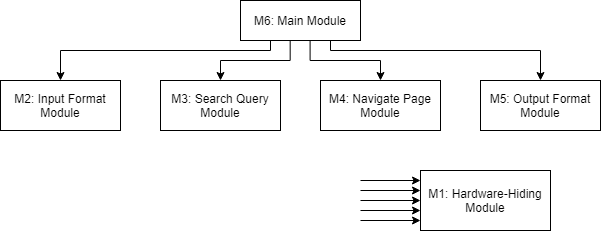
\includegraphics[width=0.9\textwidth]{UsesHierarchy.png}
\caption{Use hierarchy among modules}
\label{FigUH}
\end{figure}

%\section*{References}

\bibliographystyle {plainnat}
\bibliography {MG}

\end{document}